\documentclass[
	% -- opções da classe memoir --
	12pt,				% tamanho da fonte
	openright,			% capítulos começam em pág ímpar (insere página vazia caso preciso)
	oneside,			% para impressão em verso e anverso. Oposto a oneside
	a4paper,			% tamanho do papel.
	% -- opções da classe abntex2 --
	%chapter=TITLE,		% títulos de capítulos convertidos em letras maiúsculas
	%section=TITLE,		% títulos de seções convertidos em letras maiúsculas
	%subsection=TITLE,	% títulos de subseções convertidos em letras maiúsculas
	%subsubsection=TITLE,% títulos de subsubseções convertidos em letras maiúsculas
	% -- opções do pacote babel --
	english,			% idioma adicional para hifenização
	french,				% idioma adicional para hifenização
	spanish,			% idioma adicional para hifenização
	brazil				% o último idioma é o principal do documento
	]{abntex2}

% ---
% Pacotes básicos
% ---
\usepackage{lmodern}			% Usa a fonte Latin Modern
\usepackage[T1]{fontenc}		    % Selecao de codigos de fonte.
\usepackage[utf8]{inputenc}		% Codificacao do documento (conversão automática dos acentos)
\usepackage{lastpage}			% Usado pela Ficha catalográfica
\usepackage{indentfirst}		    % Indenta o primeiro parágrafo de cada seção.
\usepackage{color}				% Controle das cores
\usepackage{graphicx}			% Inclusão de gráficos
\usepackage{microtype} 			% Para melhorias de justificação
\usepackage{afterpage}
\usepackage{amsmath}            % Pacote para fórmulas matemáticas
\usepackage{amssymb,url}
\usepackage{xcolor,tikz,bm,colortbl}
\usepackage[br]{nicealgo}       % Pacote para criação de algoritmos
\usepackage{customizacoes}

% ---

% ---
% Pacotes adicionais, usados apenas no âmbito do Modelo Canônico do abnteX2
% ---
\usepackage{lipsum}				% Para geração de dummy text
% ---

% ---
% Pacotes de citações
% ---
\usepackage[brazilian,hyperpageref]{backref}	 % Paginas com as citações na bibl
\usepackage[alf]{abntex2cite}	% Citações padrão ABNT
% ---
% CONFIGURAÇÕES DE PACOTES
% ---

% ---
% Configurações do pacote backref
\renewcommand{\familydefault}{\sfdefault}
% Usado sem a opção hyperpageref de backref
\renewcommand{\backrefpagesname}{Citado na(s) página(s):~}
% Texto padrão antes do número das páginas
\renewcommand{\backref}{}
% Define os textos da citação
\renewcommand*{\backrefalt}[4]{
	\ifcase #1 %
		Nenhuma citação no texto.%
	\or
		Citado na página #2.%
	\else
		Citado #1 vezes nas páginas #2.%
	\fi}%
% ---

% ---
% Informações de dados para CAPA e FOLHA DE ROSTO
% ---
\titulo{Métodos de Compressão de Imagem}
\autor{Hugo Cicarelli}
\local{Bauru}
\data{2018}
\orientador{Prof. Dra. Simone das Graças Domingues Prado}
\instituicao{%
  Universidade Estadual Paulista ``Júlio de Mesquita Filho''
  \par
  Faculdade de Ciências
  \par
  Ciência da Computação}
\tipotrabalho{Trabalho de Conclusão de Curso}
% O preambulo deve conter o tipo do trabalho, o objetivo,
% o nome da instituição e a área de concentração
\preambulo{Trabalho de Conclusão de Curso do Curso de Ciência da Computação da Universidade Estadual Paulista ``Júlio de Mesquita Filho'', Faculdade de Ciências, Campus Bauru.}
% ---


% ---
% Configurações de aparência do PDF final

% alterando o aspecto da cor azul
\definecolor{blue}{RGB}{41,5,195}

% informações do PDF
\makeatletter
\hypersetup{
     	%pagebackref=true,
		pdftitle={\@title},
		pdfauthor={\@author},
    	pdfsubject={\imprimirpreambulo},
	    pdfcreator={LaTeX with abnTeX2},
		pdfkeywords={abnt}{latex}{abntex}{abntex2}{trabalho acadêmico},
		colorlinks=true,       		% false: boxed links; true: colored links
    	linkcolor=black,          	% color of internal links
    	citecolor=black,        		% color of links to bibliography
    	filecolor=magenta,      		% color of file links
		urlcolor=black,
		bookmarksdepth=4
}
\makeatother
% ---

% ---
% Espaçamentos entre linhas e parágrafos
% ---

% O tamanho do parágrafo é dado por:
\setlength{\parindent}{1.3cm}

% Controle do espaçamento entre um parágrafo e outro:
\setlength{\parskip}{0.2cm}  % tente também \onelineskip

% ---
% compila o indice
% ---
\makeindex
% ---

% ----
% Início do documento
% ----
\begin{document}

% Seleciona o idioma do documento (conforme pacotes do babel)
%\selectlanguage{english}
\selectlanguage{brazil}

% Retira espaço extra obsoleto entre as frases.
\frenchspacing

% ----------------------------------------------------------
% ELEMENTOS PRÉ-TEXTUAIS
% ----------------------------------------------------------
% \pretextual

% ---
% Capa
% ---
\imprimircapa
% ---

% ---
% Folha de rosto
% (o * indica que haverá a ficha bibliográfica)
% ---
\imprimirfolhaderosto*
% ---

% ---
% Inserir a ficha bibliografica
% ---

% Isto é um exemplo de Ficha Catalográfica, ou ``Dados internacionais de
% catalogação-na-publicação''. Você pode utilizar este modelo como referência.
% Porém, provavelmente a biblioteca da sua universidade lhe fornecerá um PDF
% com a ficha catalográfica definitiva após a defesa do trabalho. Quando estiver
% com o documento, salve-o como PDF no diretório do seu projeto e substitua todo
% o conteúdo de implementação deste arquivo pelo comando abaixo:
%
% \begin{fichacatalografica}
%     \includepdf{fig_ficha_catalografica.pdf}
% \end{fichacatalografica}

\begin{fichacatalografica}
	\sffamily
	\vspace*{\fill}					% Posição vertical
	\begin{center}					% Minipage Centralizado
	\fbox{\begin{minipage}[c][8cm]{15.5cm}		% Largura
	\small
	\imprimirautor
	%Sobrenome, Nome do autor

	\hspace{0.5cm} \imprimirtitulo  / \imprimirautor. --
	\imprimirlocal, \imprimirdata-

	\hspace{0.5cm} \pageref{LastPage} p. : il. (algumas color.) ; 30 cm.\\

	\hspace{0.5cm} \imprimirorientadorRotulo~\imprimirorientador\\

	\hspace{0.5cm}
	\parbox[t]{\textwidth}{\imprimirtipotrabalho~--~\imprimirinstituicao,
	\imprimirdata.}\\

	\hspace{0.5cm}
		1. Image Compression
		2. Lossless
		3. Lossy
		4. Open Source
		I. \imprimirorientador.
		II. Universidade Estadual Paulista "Júlio de Mesquita Filho".
		III. Faculdade de Ciências.
		IV. Métodos Compressão de Imagem
	\end{minipage}}
	\end{center}
\end{fichacatalografica}
% ---

% ---
% Inserir folha de aprovação
% ---

% Isto é um exemplo de Folha de aprovação, elemento obrigatório da NBR
% 14724/2011 (seção 4.2.1.3). Você pode utilizar este modelo até a aprovação
% do trabalho. Após isso, substitua todo o conteúdo deste arquivo por uma
% imagem da página assinada pela banca com o comando abaixo:
%
% \includepdf{folhadeaprovacao_final.pdf}
%
\begin{folhadeaprovacao}

  \begin{center}
    {\ABNTEXchapterfont\large\imprimirautor}

    \vspace*{\fill}\vspace*{\fill}
    \begin{center}
      \ABNTEXchapterfont\bfseries\Large\imprimirtitulo
    \end{center}
    \vspace*{\fill}

    \hspace{.45\textwidth}
    \begin{minipage}{.5\textwidth}
        \imprimirpreambulo
    \end{minipage}%
    \vspace*{\fill}
   \end{center}

   \center Banca Examinadora

   \assinatura{\textbf{\imprimirorientador} \\ Orientador}
   \assinatura{\textbf{Prof. Dra. Simone das Graças Domingues Prado} }
   \assinatura{\textbf{Prof. Dra. Andrea Carla } }

   \begin{center}
    \vspace*{0.5cm}
    \par
    {Bauru}
    {2018}
    \vspace*{1cm}
  \end{center}

\end{folhadeaprovacao}
% ---

% ---
% Dedicatória
% ---
\begin{dedicatoria}
   \vspace*{\fill}
   \centering
   \noindent
   \textit{Espaço destinado à dedicátoria do texto.} \vspace*{\fill}
\end{dedicatoria}
% ---

% ---
% Agradecimentos
% ---
\begin{agradecimentos}
Espaço destinado aos agradecimentos.
\end{agradecimentos}
% ---

% \textemdash
% Epígrafe
% ---
\begin{epigrafe}
    \vspace*{\fill}
	\begin{flushright}
		\textit{Espaço destinado à epígrafe.}
	\end{flushright}
\end{epigrafe}
% ---

% ---
% RESUMOS
% ---

% resumo em português
\setlength{\absparsep}{18pt} % ajusta o espaçamento dos parágrafos do resumo
\begin{resumo}

Espaço destinado à escrita do resumo.

\textbf{Palavras-chave:} Palavras-chave de seu resumo.
\end{resumo}

% resumo em inglês
\begin{resumo}[Abstract]
 \begin{otherlanguage*}{english}

Abstract area.

\textbf{Keywords:} Abstract keywords.

 \end{otherlanguage*}
\end{resumo}
% ---

% ---
% inserir lista de ilustrações
% ---
\pdfbookmark[0]{\listfigurename}{lof}
\listoffigures*
\cleardoublepage
% ---

% ---
% inserir lista de tabelas
% ---
\pdfbookmark[0]{\listtablename}{lot}
\listoftables*
\cleardoublepage
% ---

% ---
% inserir lista de abreviaturas e siglas
% ---
% ---

% ---
% inserir o sumario
% ---
\pdfbookmark[0]{\contentsname}{toc}
\tableofcontents*
\cleardoublepage
% ---



% ----------------------------------------------------------
% ELEMENTOS TEXTUAIS
% ----------------------------------------------------------
\pagestyle{simple}

% ----------------------------------------------------------
% Introdução (exemplo de capítulo sem numeração, mas presente no Sumário)
% ----------------------------------------------------------

\chapter{Introdução}
\label{c.introducao}

Compressão de imagem permite reduzir seu tamanho em disco, buscando a menor perda de qualidade possível. A busca por isso se dá, por exemplo, caso se queira acessar um site em um dispositivo móvel. O número de celulares acessando sites tem crescido bastante nos últimos anos. De acordo com o site Statista.com (https://www.statista.com/topics/779/mobile-internet/ - acessado em 27/05/2018), em 2018, o tráfico de internet acessado por celulares foi de 51.2\% em todo o globo. Tendo isso em mente, ao acessar um site contendo uma imagem em seu tamanho original, pode-se levar um tempo 5 vezes maior do que ao comprimi-la.

O tópico sobre compressão de imagens tem ganhado grande destaque por conta de perfomance, como também no quesito de armazenamento em disco. Para sanar a necessidade de falta de espaço em disco surgiram novas tecnologias, que é o caso dos Serviços em Nuvem. Esses Serviços permitem que sejam alocados recursos computacionais, cobrando um valor em cima do que se é realmente utilizado. Embora isso sane em parte o problema de armazenamento, ainda se é investido tecnologias e tempo para otimizar arquivos de imagens, pois reflete em um maior número de imagens em um servidor na nuvem pelo mesmo preço.

\section{Problema}
\label{s.problema}

Acessos por celulares nem sempre são feitos através de redes de internet WiFi, sendo muitas das vezes sendo acessados pela rua através de redes 3G/4G. Isso se torna um problema no consumo de dados, ao fazer requisição para arquivos muito grandes, além da demora para ser mostrada uma imagem, muitas vezes renderizadas em dimensões muito menor que a original.

Outro problema se dá que para se otimizar qualquer tipo de arquivo, é necessário que alguma informação seja removida. Por isso, precisa-se escolher o que se busca de fato: tamanho em disco ou qualidade da imagem.

Existem métodos, os quais iremos abortar, que tratam a otimização buscando sempre a menor perda de qualidade, ou dimensões da imagem. Seu uso irá variar com o que o usuário final busca.
\chapter{Objetivos}
\label{c.objetivos}

\section{Objetivos Gerais}
\label{s.objetivosgerais}

Têm-se como objetivo final a criação de um aplicativo de Compressão de Imagens, o qual irá oferecer para o usuário o melhor cenário para o que se deseja, seja qualidade da imagem ou redimensionando-a.

\section{Objetivos Específicos}
\label{s.objetivosespecificos}

\begin{alineas}
	\item Aprender metodologias de compressão de imagem;
	\item Aprender algoritmos que permitem implementar as metodologias apresentadas;
	\item Melhorar habilidades com a linguagem PHP;
\end{alineas}

\chapter{Fundamentação Teórica}
\label{c.fundamentacaoteorica}

Em Ciência da Computação, compressão de dados é o processo de codificar as mesmas informações usando um número menor de bits, sem que haja distorção dos dados originais. Em se tratando de compressão de imagens, pode-se alcançar Esse processo é útil, pois reduz o consumo de recursos computacionais, como espaço em disco, ou utilização de banda de internet.

Considere as imagens abaixo.

\begin{figure}[h]
\caption{\small Codificador e Decodificado de Imagens}
\centering
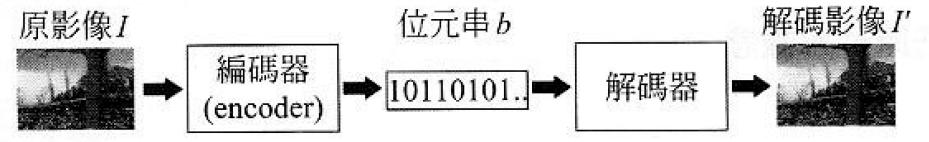
\includegraphics[scale=0.50]{figs/image_compression.jpg}
\label{f.imagecompressionbasics}
\legend{\small Fonte: Elaborada pelo autor.}
\end{figure}

Quando o sistema recebe a imagem original, ele manda para um codificador que converte a imagem original para um fluxo de bits. Um decodificador então recebe esse fluxo de bits e o transforma novamente na imagem. Caso o fluxo de bits final seja menor que o original, chamamos esse processo de Compressão de Imagem.

\citeauthor{mackenzielossless} diz que durante a compressão de uma imagem, pode-se ter perda de dados durante o processo. Por essa razão, o decodificador não consegue reconstruir a imagem perfeitamente para seu estado inicial. Esse tipo de compressão é chamado de Lossy, e esse processo é irreversível. O processo no qual a imagem pode retornar ao seu estado inicial é chamado de {\em Lossless}, o qual é possível reduzir o tamanho em disco, sem ter perda de dados durante o processo, sendo esse um processo reversível.

\section{Métodos de Compressão de Imagem Sem Perda}
\label{s.lossless}

São os chamados tipos de compressão {\em Lossless}. Neles, como dito anteriormente, é possível restaurar todos os dados originais da Imagem ao descompacta-la. Esse tipo de compressão é geralmente usado para arquivos de imagem de extensão GIF, formato usado na internet o qual são permitidas animação de imagens e utilização de transparência.

De acordo com \citeauthor{losslessmethods} define que compressão de imagens do tipo {\em Lossless}, também conhecidas como Compressão de Imagem Sem Perda, podem ser alcançadas através de Métodos de Codificação, Domínio Espacial, Domínio de Frequência, os quais são baseados em Transformadas, são uma combinação desses métodos.

Métodos de codificação são diretamente aplicados a imagens de formato RAW, o qual é o formato mais puro de uma imagem, normalmente sendo gerado a partir de câmeras profissionais. Esse formato acumula todos os dados necessários da imagem, como abertura da câmera, tipo da câmera, ISO utilizada, entre outras informações. O método de codificação trata a imagem como uma sequência de números discretos. Métodos comuns dessa incluem aritmética, Huffman, Lempel-Ziv Welch e Run-Length.

Métodos de domínio espacial são uma combinação de algoritmos de domínio espacial e métodos de codificação. Eles não somente operam diretamente nos tons de cinza, que são tons atribuidos a um pixel sendo 0 equivalente a branco e 100 equivalente a preto, como também tentam eliminar a redundância espacial. Essa redundância consiste na semelhança de pixels adjacentes de uma imagem. Suponhamos o seguinte exemplo: uma imagem de um avião passando no céu sem nuvens, na qual a informação relevante a ser transmitida é o avião, e o fundo é a parte da imagem azul cujo conteúdo da imagem é praticamente uniforme.

Na compressão de domínos de frequência, a imagem é representada usando uma base apropriada, com o objetivo de se obter um coeficiente de matriz pequeno. Transformada do Cosseno Discreto (DCT) e Transformada Wavelet são exemplos de compressão de domínio de frequência.

\subsection{Performance}
\label{ss.losslessperformance}

Perfomance em algoritmos do tipo {\em Lossless} pode ser especificados em termos de complexidade e eficiência.

A complexidade de um algoritmo de compressão de imagem é medida pelo número de operações aritméticas necessárias para realizar ambos processos de codificação e decodificação. Esse é um fator importante para aplicações que envolvem compressão online, onde a velocidade é crucial.

Eficiência de compressão é medida pela proporção de compressão ou pela taxa de bits. Proporção de compressão é o número de bits por pixel de uma imagem comprimida. Por exemplo, se uma imagem de dimensões 256x256 de 8 bits por pixel, é necessários 256 * 256 * 8 bits = 65.536 bytes quando armazenada em sua forma original. Se a imagem otimizada possuir 32.768 bytes, então a proporção de compressão será 65536 / 32768 = 2. Como a imagem possui dimensão de 256x256 = 65.536 pixels, o arquivo comprimido precisa de 32768 * 8 / 65536 = 4 bits, o qual será a taxa de bits necessária. A proporção de compressão portanto está associada a taxa de bits necessária. Sendo {\em CR} a proporção de compressão, {\em BR} a taxa de bits e {\em v} o número de bits por pixel de uma imagem não otimizada, temos a seguinte fórmula:

\[ CR = b / BR \]

\subsection{Métodos de Codificação}
\label{ss.codingmethod}

Nessa seção, serão abordados alguns algoritmos de codifição, bem como a explicação do método.

Para casos de codificação na qual uma imagem em duas dimensões será comprimida, existe a necessidade de convertê-la para uma sequência de uma dimensão. Para esse processo, chamamos de Linearização.

\subsubsection{Linearização}
\label{sss.linearlization}

A linearização não afeta a frequência da codificação, sendo esse método aplicado para alguns casos. Como Huffman depende somente da frequência dos diferentes tons de cinza, o método não é afetado pela linearização. Agora métodos como Liv-Zempel dependem da ordem dos tons de cinza, sendo então afetados por métodos de linearização.

Imagens possuem o que é chamado de redundância local, o que causa uma certa região da imagem a exibir uma coerência ou correlação, resultando em uma suavidade entre os pixels. Alguns métodos de linearização são mais efetivos que outros em se tratando de preservar essa região e, por isso, são esperados terem melhor desempenho quando combinadas com métodos de codificação que se utilizam dessas regiões de redundância.

Abaixo está uma lista dos métodos de linearização mais utilizados, segundo \citeauthor{losslessmethods}:

\begin{alineas}
    \item Verificação orientada por linha ({\em Row-Major Scan}): a imagem é verificada linha por linha, sentido cima-esquerda para baixo-direita;
    \item Verificação orientada por coluna ({\em Column-Major Scan}): a imagem é verificada coluna por coluna, com sentido cima-esquerda para baixo-direita;
    \item Verificação orientada por diagonal ({\em Diagonal Scan}): a imagem é verificada em diagonais, começando do canto inferior esquerdo para o canto superior direito;
    \item Verificação em formato de cobra ({\em Snake-like row-major Scan}): é uma variação da verificação orientada por linhas e orientada por colunas. Nela, ao chegar no final de uma linha, segue para a linha de baixo continuando na mesma coluna;
    \item Verificação em espiral ({\em Spiral Scan}): nesse método,;
    \item Verificação de Peano-Hilbert ({\em Peano-Hilbert Scan}): essa verificação requer que a imagem seja \[ 2^k * 2^k \]. Quando {\em k} é ímpar, o caminho percorrido começa no pixel mais a esquerda da primeira linha e termina no pixel mais a esquerda da última linha. Quando {\em k} é par, o caminho começa no pixel mais a esquerda da primeira linha e termina no pixel mais a direita da última linha.;
\end{alineas}

Segundo o autor, embora que nenhum método de linearização forneça a melhor compressão, a verificação de Peano-Hilbert geralmente traz o melhor resultado.

\subsubsection{Codificação de Huffman}
\label{sss.huffmancoding}

Nesse método, a redundância de codificação é eliminada com base numa codificação que produz um código de tamanho variável, atribuindo os códigos de tamanhos menores aos níveis de cinza mais prováveis de ocorrer.

Esse método possui duas etapas:

\begin{alineas}
    \item Cria-se uma série de reduções dos símbolos através da junção dos dois de menores probabilidades a cada iteração.
    \item Codificam-se todos os símbolos que foram reduzidos, começando com o de maior probabilidade que será associado ao menor código e voltando para os originais.
\end{alineas}

\citeauthor{losslesscodings} dá o seguinte exemplo: imagem de tamanho 10x10 e 6 tons de cinza (a1, a2, a3, a4, a5, a6), tendo as seguintes probabilidades de ocorrência: 5/8 de a1, 3/32 de a2 e a3, 1/32 de a6 e a4, e 1/8 de a5.

\begin{figure}[h]
\caption{\small Primeira etapa de codificação de Huggman.}
\centering
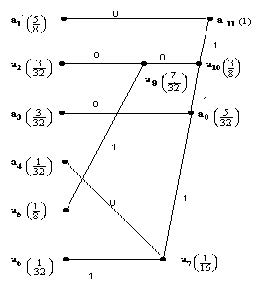
\includegraphics[scale=0.50]{figs/huffman_etapa1.jpg}
\label{f.huffmanetapa1}
\end{figure}

Tabela referente a segunda etapa da codificação de Huffman para as probabilidades das palavras mostradas na figura anterior.

\begin{table}[]
    \begin{center}
        \caption{\small Segunda etapa da codifiçãode Huggman}
        \label{t.huffmanetapa2}
        \begin{tabular}{llr}
            Informação & Probabilidade & Código \\
            a1         & 5/8 = 20/32   & 0      \\
            a10        & 3/8 = 12/32   & 1      \\
            a9         & 7/32          & 10     \\
            a8         & 5/32          & 11     \\
            a5         & 1/8 = 4/32    & 101    \\
            a2         & 3/32          & 100    \\
            a3         & 3/32          & 110    \\
            a7         & 2/32          & 111    \\
            a4         & 1/32          & 1110   \\
            a6         & 1/32          & 1111
        \end{tabular}
    \end{center}
\end{table}

Para transmitir essa informação, obtem-se uma taxa média de bits/informação seguindo a seguinte fórmula:

\[ (5/8)*1 + (3/32)*3 + (3/32)*3 + (4/32)*3 + (1/32)*4 + (1/32)*4 = 1,813 \] {\em bits}/informação.

\subsubsection{Codificação por LZW}
\label{sss.lzw}

Lempel, Ziv e Welch propuseram um método de codificação adaptável que não requer que todos que irão ser compressados, estejam disponíveis desde o começo. Essa técnica gera o código conforme o vai examinando, do começo ao fim. Na codificação por Huffman, um código de tamanho variável é construído para cada símbolo no código fonte. Na codificação Lampel-zev, códigos de tamanho fixo são construídos a medida que o processo vai rodando, para cada sequência de símbolos de tamanho variável.

Suponhamos que os símbolos que ocorrem em um código seja {\em a}, {\em b}, e {\em c}, e que a cadeia de caracteres {\em ababcabc} está para ser comprimida. Primeiro, iniciamos o dicionário para essa tradução no qual apenas um símbolo seja possível. Como o código do dicionário é dado pela posição, {\em a} seria 0, {\em b} seria 1 e {\em c} seria 2. Ao ler a cadeia de caracteres ababcabc, temos o primeiro sendo {\em a}. Seu código 0 seria parte do arquivo comprimido em conjunto com o prefixo e a próxima entrada. Nesse caso, seria {\em ab} e o código seria 3. A parte que restou para compressão agora seria {\em babcabc}. Novamente pegamos a cadeia de maior prefix que sobrou, sendo {\em b} nesse caso. Seu código é 1, somando com o próximo prefixo que é {\em a}, temos o código 4. Como agora temos no dicionário os caracteres {\em a} e {\em b}, a próxima sequência que pegaremos da cadeia restante, {\em abcabc} será {\em ab}. O código dela é 3, somando com o código do próximo caracter {\em c}, temos o valor 5. Como próxima sequência encontrada é {\em c}, com código 2 e temos {\em ca} entrando no dicionário. A cadeia restante então é {\em abc}, a qual está no dicionário, com valor 5. Com isso, foi possível chegar na codificação da cadeia {\em ababcabc}, a qual é 01325.

O método de compressão gzip, utilizado por sistemas Unix, utiliza uma combinação dos métodos de Huffman e LZW.

\subsubsection{Codificação por Código de Tons Corridos (RLE)}
\label{sss.runlength}

Nesse método, o código fonte é dividido em segmentos de símbolos idênticos. Cada segmento é separado por um símbolo e o número de ocorrências.

Para elucidar, suponha a cadeia {\em aaaabaaabb}. Ela é codificada como (a, 4), (b, 1), (a, 3), (b, 3). Esse método de codificação funcional bem para cadeias que possuem segmentos grandes, como imagens com fundos uniformes, porém esse método não é tão eficaz quando as cadeias possuem muitos segmentos curtos

\subsection{Métodos de Domínio Espacial}
\label{ss.transformmethod}

\citeauthor{pasteldeflango} diz que os algoritmos de domínio espacial envolvem métodos para reduzir o número de bits que representam a informação contida na imagem operando diretamente em seu formato mais cru, o qual contém maior número de informações. Tais métodos geralmente envolvem duas etapas. O primeiro estágio envolve o uso de técnicas como segmentação de imagem, amostras e interpolarização. Essa etapa é seguida por uma aproveita eficientemente as codificações produzidas pela primeira etapa.

Na primeira etapa, técnicas de segmentação de imagem incluem métodos de partição da imagem em formatos regulares, tais como retângulos, os quais ocupam menor armazenamento para codificar o formato devido a simplicidade, mas também podem assumir formatos irregulares, sendo esses últimos possuem um maior armazenamento devido a complexidade dos formatos resultantes do algoritmo de segmentação. Formatos mais simples necessitam de poucos bits para codificar a forma, mas possuem a restrição na representação, tendo um maior número de formas mais simples para representar a imagem total.

Muitos algoritmos dessa técnica são usadas nos métodos de compressão {\em Lossy}.

\subsubsection{Compressão de Tamanho de Bloco Variável}
\label{sss.variableblock}

\subsubsection{Abordagem residual + Lossy}
\label{sss.lossyresidual}

\subsubsection{Algoritmos de Compreesão Contextuais}
\label{sss.contextbased}

\subsection{Métodos de Domínio de Frequência}
\label{ss.transformmethod}

% \chapter{Metodologia}
\label{c.metodologia}

\section{Métodos e Etapas}
\label{s.metodoseetapas}

Para o desenvolvimento do projeto foi realizado o levantamento bibliográfico de metodologias existentes para realizar Testes de Penetração, analisando seus diversos aspectos e quais nos auxiliariam melhor em nosso objetivo, bem como modos de como aplicá-las em Sistemas na Nuvem..

Com a base teórica definida a etapa seguinte foi aplicar uma estrutura modular que correspondesse ao modelo teórico, para que todas as etapas da extração e reconhecimento do \emph{audio fingerprint} possam ser modificadas sem que alterem o funcionamento geral do processo. Essa estrutura adaptável foi aplicada com base no modelo teórico genérico de reconhecimento de áudio.

% A terceira e última etapa foi o desenvolvimento de uma aplicação de reconhecimento específico de músicas, utilizando um cálculo de \emph{audio fingerprint} baseado em representações que levam em conta a repetição de refrões através da análise baseada em altura tonal e \emph{chroma} musical.

\section{Materiais Utilizados}
\label{s.materiaisutilizados}

\subsection{Ambiente de desenvolvimento}
\label{s.kali}

Para desenvolvimento do projeto foi utilizado o Sistema Operacional Kali Linux, uma distribuição Linux especializada em Testes de Intrusão e Auditoria de Segurança.

\subsection{Github}
\label{s.github}

O Github é ao mesmo tempo um servidor de armazenamento de código e uma rede social onde pode-se submeter modificações, fazer cópias e acompanhar modificações de códigos de outras pessoas. A rede foi essencial para o desenvolvimento deste projeto por armazenar vários sub-módulos e disponibilizar código-fonte para consulta.

% \chapter{Desenvolvimento}
\label{c.desenvolvimento}

\section{Utilizando Métodos {\em LossLess}}
\label{s.losslessdev}

Para o método sem perda escolhido foi a Codificação de Huffman, por ser uma técnica simples e fácil de aplicar. A técnica, como descrita no Capítulo 2, se baseia em remover a redundância de bits ao analisar diferentes características ou especificações.

\subsection{Codificação de Huffman}
\label{ss.huffmandev}

O primeiro passo nessa técnica é de reduzir a imagem original em um histograma ordenado, onde a probabilidade de ocorrência de um certo valor de intensidade de um pixel é igual a \[ PP = NP / T \] onde {\em PP} é a probabilidade de ocorrência, {\em NP} é o número de pixels de mesma intensidade e {\em T} o número total de pixels contidos na imagem original.

Histograma é a representação gráfica em colunas ou em barras de um conjunto de dados previamente tabulado e dividido em classes uniformes ou não uniformes.

Dada a seguinte imagem:

\begin{figure}[h]
\caption{\small Imagem 8x8 pixels}
\centering

\includegraphics[scale=0.50]{figs/Input-Image-1.png}
\label{f.imagecompressionbasics}
\end{figure}

Ao se fazer seu histograma, temos:

\begin{table}[]
    \begin{center}
        \caption{\small Valores de intensidade de pixels}
        \label{t.imagecompressionbasics}
        \begin{tabular}{llrlllll}
            128 & 75  & 72  & 105 & 149 & 169 & 127 & 100 \\
            122 & 84  & 83  & 84  & 146 & 138 & 142 & 139 \\
            118 & 98  & 89  & 94  & 136 & 96  & 143 & 188 \\
            122 & 106 & 79  & 115 & 148 & 102 & 127 & 167 \\
            127 & 115 & 106 & 94  & 115 & 124 & 103 & 155 \\
            125 & 115 & 130 & 140 & 170 & 174 & 115 & 136 \\
            127 & 110 & 122 & 163 & 175 & 140 & 119 & 87  \\
            146 & 114 & 127 & 140 & 131 & 142 & 153 & 93
        \end{tabular}
    \end{center}
\end{table}

A imagem contém 46 valores de intensidade distintos, portanto terá 46 símbolos únicos no dicionário de Huffman.

O método de Huffman pode ser separado da seguinte forma:

\begin{alineas}
    \item Ler a imagem como um vetor 2D
    \item Definir a estrutura que irá conter os valores de intensidade
    \item Definir outra estrutura que irá
\end{alineas}

\subsubsection{Ler a imagem como um vetor 2D}
\label{sss.imagetoarray}

Primeiramente, temos que transformar a imagem em um vetor 2D. Para isso, utilizamos a seguinte função em PHP:

\begin{verbatim}
public function image_to_array( $image ) {
    $width = imagesx($image);
    $height = imagesy($image);
    $colors = array();

    // percorre os pixel por coluna
    for  ($y = 0; $y < $height; $y++ ) {
        // percorre os pixels por linha
        for ($x = 0; $x < $width; $x++) {
            // retorna o índice da cor de um pixel no local especificado
            $rgb = imagecolorat($image, $x, $y);
            $r = ($rgb >> 16) & 0xFF;
            $g = ($rgb >> 8) & 0xFF;
            $b = $rgb & 0xFF;

            $black = ($r == 0 && $g == 0 && $b == 0);
            $colors[$x][$y] = $black;
        }
    }
}
\end{verbatim}

% \chapter{Conclusão}
\label{c.conclusao}

Tendo-se em mente os métodos estudados de compressão sem perda, o método de Huffman foi escolhido por ter sua aplicação simples e fácil, e um ponto importante foi a falta de pantente, tornando a utilização desse método em aplicações comerciais sem nenhum custo.

Embora o algoritmo desse método seja ótimo para codificação símbolo a símbolo com uma distribuição de probabilidade conhecida, quando este caso não ocorre, não se torna tão vantajoso assim. Esse método pode ser utilizado em conjunto com outros, para garantir um melhor desempenho. Ferramentas de compactação, como o GZIP, se utilizam disso para realizar as compressões em sistemas Linux.

Durante o desenvolvimento, foram encontradas dificuldades durante o processo, principalmente para retornar ao estado de uma imagem, decodificando os resultados da Árvore de Huffman.

Atualmente, a busca por maior compressão de itens estáticos, como imagens, tem aumentado e muito. Com esse fator, o número de ferramentas disponíveis para tal tem aumentado também, porém a taxa de compressão é variada, sempre tendo uma busca pelo que melhor se adapa ao desejado. Ferramentas como TinyPNG, utilizada durante a fase de testes e comparação, ou Cloudinary, aplicação online a qual permite hospedagem de imagens e arquivos estáticos bem como sua otimização tanto na qualidade, como também usando métodos de recorte o qual também diminui seu espaço em disco, são amplamente usadas no dia a dia, tanto de aplicações mais gerais, como também de sites e blogs pela internet.



% ----------------------------------------------------------
% ELEMENTOS PÓS-TEXTUAIS
% ----------------------------------------------------------
\postextual
% ----------------------------------------------------------

% ----------------------------------------------------------
% Referências bibliográficas
% ----------------------------------------------------------
\pagestyle{empty}
\bibliography{references} % o arquivo de bibliografia deve ser importando nessa linha sem o .bib

% ----------------------------------------------------------
% Glossário
% ----------------------------------------------------------
%
% Consulte o manual da classe abntex2 para orientações sobre o glossário.
%
%\glossary

%---------------------------------------------------------------------
% INDICE REMISSIVO
%---------------------------------------------------------------------
\phantompart
\printindex
%---------------------------------------------------------------------

\end{document}
